\documentclass[conf]{new-aiaa}
%=============================================================
\usepackage{graphicx}
\usepackage{amsmath}
\usepackage[version=4]{mhchem}
\usepackage{siunitx}
\usepackage{bm}
\usepackage{scalerel}
\usepackage{tikz,pgfplots,pgfplotstable}
\usepackage{subcaption}
\usepackage[abs]{overpic}
\usepackage{mathtools}
%=============================================================
\linespread{1.4}
%=============================================================
\DeclareMathAlphabet{\mathesstixfrak}{U}{esstixfrak}{m}{n}
\DeclareMathAlphabet{\mathboondoxfrak}{U}{BOONDOX-frak}{m}{n}
\newcommand{\ie}{\emph{i.e~}}
\renewcommand{\th}{\textsuperscript{th}~}
\DeclareMathOperator{\Nabla}{\mathbf{\nabla}}
\newcommand{\HRule}{\rule{\linewidth}{0.5mm}} %To use HRule command
\newcommand*{\acro}[1]{\textsc{\MakeLowercase{#1}}} % acronyms etc.
\newcommand*{\unit}[1]{\ensuremath{\,\mathrm{#1}}}
\newcommand*{\pd}[3][]{\frac{\partial^{#1}#2}{\partial{#3}^{#1}}} % partial derivative
\newcommand*{\reyno}[1]{\bar{#1}}
\newcommand*{\favre}[1]{\widetilde{#1}}
\newcommand{\ud}{\mathrm{d}} 
\newcommand{\uD}{\mathrm{D}}
\newcommand*{\dwz}{\delta_{\omega,0}}
\newcommand*{\dw}{\delta_{\omega}}
\newcommand{\pars}[1]{\left(\,{#1}\,\right)}
\newcommand*{\uunit}[1]{\ensuremath{\mathrm{#1}}}
\newcommand*{\ex}[1]{\times 10^{#1}}%shorthand -- for use in tables
\newcommand{\adinf}[1]{{#1}_{\mathrm{\infty}}} % infinity
\newcommand{\adinfb}[1]{{#1}^*_{\mathrm{\infty}}} % infinity b
\newcommand{\adref}[1]{{#1}_{\mathrm{ref}}} % reference
\newcommand{\adrefb}[1]{{#1}^*_{\mathrm{ref}}} % reference b
\newcommand{\adndim}[1]{{#1}^*} % non-dimensioned
\newcommand{\addim}[1]{{#1}} % dimensioned
\newcommand{\Wcal}{\mathcal{W}}
\newcommand{\Rcal}{\mathcal{R}}
\newcommand{\nspc}{\mathcal{N}_{sp}}
\newcommand{\w}{\mathcal{W}}
\newcommand{\ro}[1]{\mathrm{#1}}
%=============================================================
\title{A gPC-based approach to uncertain interaction of oblique shocks and supersonic mixing layers}
%=============================================================
% \setlength\LTleft{0pt} 
%=============================================================
\author{
Sarah Baaziz
\footnote{Graduate Student, sarah.baaziz@um6p.ma}}
\affil{University of Lille, Lille Fluid Mechanics Laboratory, Lille, France}
\author{Nabil El Moçayd
\footnote{Assistant professor, nabil.elmocayd@um6p.ma}}
\affil{Mohammed VI Polytechnic University (UM6P), IWRI Group, Benguerir, Morocco}
\author{Imad Kissami
\footnote{Research \& Education fellow, radouan.boukharfane@um6p.ma, AIAA Member}}
\author{Radouan Boukharfane
\footnote{Research \& Education fellow, radouan.boukharfane@um6p.ma, AIAA Member}}
\affil{Mohammed VI Polytechnic University (UM6P), MSDA Group, Benguerir, Morocco}
\begin{document}
%=============================================================
\date\today
%=============================================================
\maketitle
%=============================================================
\begin{abstract}
The present paper focus on the stochastic response of a two-dimensional shock wave impingement on a spatially evolving mixing layer to parametric uncertainties.
%
Both the oblique shock angle and the convective Mach number are considered as random parameters and the generalized Polynomial Chaos (gPC) theory is coupled with standard deterministic numerical simulations through a spectral collocation projection methodology.
%
In this framework, the two input parameters investigated are considered as random variables with a given probability distribution over the range of investigation prescribed.
%
The uncertainty is then propagated through the computational model to statistically quantify their effect on the results.
%
This study allows for a better understanding of the flow sensitivity to such uncertainties and underline the coupling process between the stochastic parameters.
%
Some results of direct numerical simulations of the multicomponent, compressible, reactive Navier-Stokes equations are reported here for the particular case of a two-dimensional mixing layer. Special emphasis is placed on the effects associated with heat release.
\end{abstract}
%=============================================================
\section{Introduction}
%=============================================================
%
The validation and verification of computational fluid dynamics (CFD) tools using wind tunnel experimental results poses many questions on the way to setup the test case and on the necessary test data to use in the numerical configuration to make the numerical simulation most compatible to the real flow \cite{szoke2020developing}.
%
In this process the account of real information on the flow generated by the wind tunnel appears as an important matter often neglected in the simulation work.
%
In fact a wind tunnel represents a complex system that generates testing conditions not necessarily well-known \cite{cattafesta2010fundamentals}.
%
This leads to an intrinsic uncertainty in the proper setting and initialisation of the numerical model to target experimental reproduction that, on general grounds, includes geometrical and flow parameters alike.
%
In this work, the system of interest is the interactions of shocks with shear flows which occur in many high-speed flow situations such as external aerodynamics of transonic, supersonic and hypersonic flow, internal flows in scramjets \cite{chakravarthy2018analytical,karthick2021shock}.
%
Shock interactions with free shear and wall-bounded flows have been shown to impact mixing, increase losses and affect surface drag and/or heat transfer depending upon the strength of the shock. 
%
Uncertainty quantification of the influence of uncertain parameters onto mixing efficiency obtained from shock/shear interactions is a major issue in order to properly predict the system response to random inputs.
%
Several benefits can be gained from such studies.
%
For example, it permits to i) take into consideration realistic safety margins depending on the solution sensitivity to the random inputs, and ii) to study the coupling process between several uncertain parameters, which can not be investigated through linearized approaches like Adjoint-state-based methods \cite{mittal2016flexible}.
%
Moreover, uncertainty quantification leads to a classification of the most influential parameters on the system response and allows for the identification of extreme behaviors under specific coupling.
%
Moreover, uncertainty quantification leads to a classification of the most influential parameters on the system response.
%
A better understanding of the related phenomena is thus required for applications such as scramjet engines, the efficiency of which depends crucially on a proper mixing of oxidizer and fuel.
%
In the present study,  the effects of a randon oblique shock angle and convective Mach number on the mean flow are examined. The influence of the turbulent structures on the global interaction is then identified, and the mixing enhancement is assessed.
%
The analysis is conducted in the light of DNS results.
%=============================================================
\section{Description of the numerical solver}
%=============================================================
The unsteady, compressible Navier-Stokes equations are considered for a multi-species reactive gas mixture:
\begin{equation}\label{eq:eqs_originelles_ch_i}
\pd{\addim{\rho}}{\addim{t}}+
\pd{\addim{\rho} \addim{u}_j}{\addim{x}_j}=0 ,
\end{equation}
\begin{equation}
\pd{\addim{\rho} \addim{u}_i}{\addim{t}}+
\pd{\addim{\rho} \addim{u}_i \addim{u}_j}{\addim{x}_j}
+\pd{\addim{p}}{\addim{x}_i}=\pd{\addim{\tau}_{ij}}{\addim{x}_j} , \quad
i \in \left[ 1,3 \right] ,
\end{equation}
\begin{equation}
\pd{\addim{\rho} \addim{e}_t}{\addim{t}}+
\pd{\left(\addim{\rho} \addim{e}_t + \addim{p} \right)\addim{u}_j}
{\addim{x}_j}=
\pd{\addim{u}_j\addim{\tau}_{ij}}{\addim{x}_j}
-\pd{\addim{q}_j}{\addim{x}_j} , \label{eq:energie_ch}
\end{equation}
\begin{equation}
\pd{\addim{\rho}Y_\alpha}{\addim{t}}+
\pd{\addim{\rho} Y_\alpha \addim{u}_j}{\addim{x}_j}=
-\pd{\addim{\rho} Y_\alpha \addim{V}_{\alpha j}}{\addim{x}_j} +
\addim{\rho} \addim{\dot{\omega}}_\alpha , \quad
\alpha \in \left[ 1,\nspc \right] ,
\label{eq:eqs_originelles_ch_f}
\end{equation}
where $\addim{\tau}_{ij}=2\addim{\mu}\left(\addim{S}_{ij} - \delta_{ij} \addim{S}_{kk} / 3 \right)$ and $\addim{S}_{ij}=\left(\partial{\addim{u}_i}/\partial{\addim{x}_j}+
\partial{\addim{u}_j}/\partial{\addim{x}_i}\right)/2$. $\addim{\rho}\addim{e}_t=\addim{\rho}{\addim{u}_i\addim{u}_i}/{2}+ \addim{\rho}\sum^{\nspc}_{\alpha=1} \addim{h}_\alpha Y_\alpha - \addim{p}$ and $\addim{h}_\alpha \left(\addim{T}_1\right) =  \Delta {\addim{h}}^0_{f\alpha} + \int^{\addim{T}_1}_{\addim{T}_0}  \addim{c}_{p\alpha} \left(\addim{T}\right) \mathrm{d} \addim{T}$. The pressure of the mixture is given by $\addim{p}=\addim{\rho}{\Rcal}\addim{T}/{\Wcal}$, with $\Wcal^{-1}=\sum^{\nspc}_{\alpha=1} {Y_\alpha}/{\Wcal_\alpha}$. $\addim{q}_j=-\addim{\lambda} \partial{\addim{T}}/\partial{\addim{x}_j} + \addim{\rho} \sum^{\nspc}_{\alpha=1}  \addim{h}_\alpha Y_\alpha \addim{V}_{\alpha j} $ and $Y_{\alpha}\addim{V}_{\alpha j} = Y_{\alpha}   \sum^{\nspc}_{\beta=1} \addim{D}_{\beta} ({\Wcal_{\beta}}/{\Wcal}) \partial{X_{\beta}}/\partial{\addim{x}_j} - \addim{D}_{\alpha} ({\Wcal_{\alpha}}/{\Wcal}) \partial{X_{\alpha}}/\partial{\addim{x}_j} $.
%
This system of conservative equations is based on the following set of independent variables: the density $\addim{\rho}$, the momentum $\addim{\rho} \addim{u}_i$, the mass fraction of the $\nspc$ species $\addim{\rho} Y_{\alpha}$ and the total energy $\addim{\rho} \addim{e}_t$.
%
Each species behaves as a thermally perfect gas with its thermodynamic properties determined from the JANAF databases~\cite{stull1971janaf}.
%
The viscosity $\addim{\mu}$ and thermal conductivity $\addim{\lambda}$ depend on the temperature of the mixture as well as its composition.
%
The mixture diffusion coefficients $\addim{D}_{\alpha}$ depend on the temperature and pressure of the mixture but the Dufour and Soret effects are not taken into account.
%
The mass production terms $\addim{\dot{\omega}}_\alpha$ are derived from a set of chemical reaction equations which are expressed in terms of an Arrhenius temperature dependence form, making possible the use of detailed chemical kinetic mechanisms.

The treatment of the advective terms in the transport equations relies on a solution-adaptive finite-difference method whereby different numerical schemes are applied for shocks and broadband turbulence.
%
Narrow regions around shock waves are treated with a nonlinear upwinding seventh-order accurate weighted essentially non-oscillatory (WENO-Z) scheme of \citet{don2013accuracy} with Roe flux splitting, whereas the underlying seventh-order upwind discretization is used elsewhere by disabling the nonlinear weights.
%
At each time step, shocks are detected based on Ducros \cite{ducros1999large} shock sensor which is activated if
\begin{equation}
\partial_i u_i>0.7\sqrt{\pars{\partial_i u_i}^2+\Omega^2},
\end{equation}
%
where $\Omega^2$ is a low-pass-filtered vorticity magnitude.
%
The viscous and molecular diffusion fluxes are discretized using eighth-order centered finite difference formulas.
%
Time integration is carried out by means of a third-order total variation diminishing (TVD) Runge--Kutta algorithm~\cite{gottlieb1998total}.
%
The time step is set such that the acoustic Courant-Friedrichs-Lewy (CFL) number does not exceed $0.5$.
%
The enthalpies and the specific heat capacities of each species are expressed as polynomial functions of temperature using the \texttt{JANAF} tables \cite{stull1971janaf}. %
The above mentioned transport coefficients, \textit{i.e.}, $\kappa$, $\mu$, $\widetilde{\mathcal{D}}_{\alpha,\beta}$ and $\tilde{\chi}_{\beta}$, which are functions of the temperature and the mixture, are evaluated using the general purpose \texttt{FORTRAN} library \texttt{EGLIB} \cite{ern2004eglib}.
%
The supersonic streams of hydrogen/air consists of nine species ($\mathrm{H_2}$, $\mathrm{O_2}$, $\mathrm{H}$, $\mathrm{O}$, $\mathrm{OH}$, $\mathrm{HO_2}$, $\mathrm{H_2O_2}$, $\mathrm{H_2O}$, $\mathrm{N_2}$).
%
To speed up the simulations of the inert cases, the intermediate species are neglected and the mass fraction of $\mathrm{N_2}$ is slightly modified to guarantee mass conservation.
%
A detailed verification of the solver may be found in \cite{boukharfane2018contribution}.
%
%=============================================================
\section{Generalized polynomial chaos}
%=============================================================
%
The main features of the generalized polynomial chaos approach are briefly recalled here; for more details we refer to \citet{ghanem2003stochastic} and \citet{le2010spectral}.
%
In the last years, this stochastic approach has been applied to turbulent flow analysis with satisfying results \cite{lucor2007sensitivity}. 
%
Define a {\it probability space} ($\Omega$,$\mathcal{A}$,$\mathcal{P}$) where $\Omega$ is the event space, $\mathcal{A} \subset 2^{\Omega}$ its $\sigma$-algebra and $\mathcal{P}$ its probability measure.
%
Being $\omega$ an element of the event space, we define a random field $X(\omega)$ such that it maps the probability space into a function space $V$, $X:\Omega \rightarrow V$.
%
In the following we will consider second-order random fields, \textit{i.e.}, those satisfying the relation ${\bf E}(X,X) < + \infty$, where ${\bf E}$ denotes the expectation of a random variable.
%
In this context, gPC is a tool allowing second-order random fields to be represented through a set of random variables ${\bf \xi}(\omega)$.
%
An approximation of the random field $X(\omega)$ is then recovered through its Galerkin projection onto a polynomial orthogonal basis taking the following form:
%
\begin{equation}
X(\omega)=a_0B_0 + \sum_{i_1=1}^{\infty}a_{i_1}B_1({ \xi_{i_1}})+ \sum_{i_1=1}^{\infty} \sum_{i_2=1}^{i_1}a_{i_1 i_2}B_2({ \xi_{i_1}, \xi_{i_2}}) + ...,
\label{EldredEq}
\end{equation}
%
where $\xi = (\xi_1, ..., \xi_N)^T$ is a N-dimensional random vector and $B_i$ is a polynomial of order $i$ depending on the $\sigma$ algebra of $\xi$.
%
This expression can be easily reformulated using a term-based indexing instead of a order-based indexing.
%
Let $\Phi_k({\bf \xi}(\omega))$ be a single polynomial, the pseudospectral approximation \eqref{EldredEq} can be written as follows:
%
\begin{equation}
X(\omega)=\sum_{k=0}^{\infty}a_k\Phi_k({\bf \xi}(\omega)),
\label{LucorEq}
\end{equation}
%
in which there is a one-to-one correspondence between $a_{i_1 \, i_2 \, \cdots \, I_n}$ and $a_k$ and between $B_n({ \xi_{i_1}, \, \xi_{i_2}, \, \cdots \,, \, \xi_{i_n}})$ and $\Phi_k({\bf \xi})$
The polynomial expansion is truncated to a finite limit and the orthogonality of the polynomials is set through the relation
%
$\langle\Phi_i \Phi_j\rangle=\langle\Phi_i^2\rangle \delta_{ij}$,
%
where $\langle\cdot,\cdot\rangle$ denotes an ensemble average.
%
This inner product is defined over the measure $W(\xi)$ of the random variables as follows:
%
\begin{equation}
\langle f(\xi)g(\xi)\rangle= \int_{\omega \in \Omega} f(\xi)g(\xi)dP(\omega)= \int f(\xi)g(\xi) W(\xi) d \xi.
\end{equation}
%
Thanks to the orthogonality of the polynomial basis, each coefficient of the Galerkin projection \eqref{LucorEq} can be recovered through the following definition:
%
\begin{equation}
a_k = \frac{\langle X,\Phi_k\rangle }{\langle \Phi_{k}^2\rangle}= \frac{1}{\langle \Phi_{k}^2\rangle}\int_{\omega \in \Omega} X \Phi_k \rho({\bf \xi}) d({\bf \xi}),
\end{equation}
%
where each inner product involves a multidimensional integral over the support range of the weighting function.
%
The integrals can be computed through different mathematical methods: considering the number of random variables investigated, the coefficients $a_k$ have been computed through Gaussian quadrature in the present work.

The polynomial family to be used must be a priori specified. The choice of the polynomials affects the speed of the convergence of the series: a unsuitable polynomial family may lead to the need of a large number of degrees of freedom to obtain a given level of accuracy (\textit{i.e.} a higher order of the polynomials), while a suitable polynomials family is able to interpolate both the input and the random variables by means of a few degrees of freedom.
%
In the case of the input, when dealing with Gaussian quadrature, an optimal family has a weight coefficient similar to the function $W$.
%
The probability density function $\texttt{PDF}$ of the random variables has been considered as \textit{uniform} leading to the choice of the Legendre polynomial family: this is a well suited choice since the inner product weighting function is directly proportional with a factor $0.5$ to the set probability density function.
%
The polynomial expansion has been limited to the third order since the contribution of fourth and higher order polynomials is negligible.
%
This leads to the use of a 20 polynomial basis to generate the error cost function over the uncertainty space. 
%
The gPC application is herein used in its non-intrusive approach, \textit{i.e.}, the variables, and more precisely the error cost functions are directly projected over the orthogonal basis spanning the random space, without any modification of the deterministic solver. 
%
The number of points to discretize each random variable space is chosen in order to recover converged integrals when computing the polynomial coefficients.
%
The polynomial expansion being truncated to the third order, $5$ points for each random variable are sufficient to compute the coefficients $a_k$.
%
%=============================================================
\section{Problem statement and computational setup}
\label{sec:physical_model_and_numerical_properties}
%=============================================================
The upper stream corresponds to the fuel inlet, \textit{i.e.}, a mixture containing hydrogen, and the bottom inlet stream to vitiated air.
%
%
A typical sketch of the corresponding computational geometry is provided in Fig.~\ref{tab:config-mel-couche-cis-1} and the main parameters relevant to the present numerical simulation are given in Tab.~\ref{tab:config-mel-couche-cis-1}.
%
Assuming equal free-stream specific heat capacity ratios, the convective Mach number may be evaluated from $M_c=(\ce{U}_1-\ce{U}_2)/(a_1+a_2)$, where $a_1$ and $a_2$ denotes  the sonic speeds of streams 1 (oxidizer inlet stream) and 2 (fuel inlet stream) respectively.
%
The values of the velocity at the inlets are $\ce{U}_1=1634$ m/s at bottom (oxidizer stream) and $\ce{U}_2$ (fuel stream) is determined once the value of $M_c$ is imposed.
%
\begin{figure}[!ht]
\centering
\begin{overpic}[scale=0.75]{./figs/schema-config.pdf}
\put(92,8){\scriptsize $\beta$}
\put(52,33){\scriptsize $\ce{U}_1$}
\put(44,90){\scriptsize $\ce{U}_2$}
\put(88,33){\scriptsize $\ce{U}_1$}
\put(81,90){\scriptsize $\ce{U}_2$}
\put(107,95){\scriptsize $x_2$}
\put(278,58){\scriptsize $x_1$}
\put(140,68){\vector(1,-1){10}}
\put(120,70){\tiny Mixing layer}
\put(235,32){\vector(1,1){10}}
\put(210,28){\tiny Transmitted shock}
\put(122,4){\vector(-1,0){10}}
\put(123,4){\tiny Shock generator}
\put(210,10){\vector(-1,1){10}}
\put(185,5){\tiny Computational domain}
\put(152,30){\vector(-1,1){10}}
\put(130,26){\tiny Incident shock}
\put(176,80){\vector(1,-1){10}}
\put(150,82){\tiny Reflected shock}
\end{overpic}
\caption{Sketch of the two-dimensional shock--mixing layer interaction geometry.}
\label{fig:fig1}
\end{figure}
%
\begin{table}[!ht]
\centering \footnotesize
\begin{tabular}{| c | c | c | c | c | c |}
\hline\hline
Simulation no. & $\beta$ ($^\circ$) & 	Mach convective $M_c$ (-) & Fuel $U_2$ (m/s) & Oxidizer $U_1$ (m/s) & ${Re_{\delta_{\omega}}}$ (-)\\ \hline\hline
1&34.24&0.45&1009.59&1634.00&602.35\\
2&34.24&0.46&994.37&1634.00&617.04\\
3&34.24&0.48&972.09&1634.00&638.52\\
4&34.24&0.50&949.82&1634.00&660.01\\
5&34.24&0.51&934.60&1634.00&674.69\\
6&35.15&0.45&1009.59&1634.00&602.35\\
7&35.15&0.46&994.37&1634.00&617.04\\
8&35.15&0.48&972.09&1634.00&638.52\\
9&35.15&0.50&949.82&1634.00&660.01\\
10&35.15&0.51&934.60&1634.00&674.69\\
11&36.50&0.45&1009.59&1634.00&602.35\\
12&36.50&0.46&994.37&1634.00&617.04\\
13&36.50&0.48&972.09&1634.00&638.52\\
14&36.50&0.50&949.82&1634.00&660.01\\
15&36.50&0.51&934.60&1634.00&674.69\\
16&37.85&0.45&1009.59&1634.00&602.35\\
17&37.85&0.46&994.37&1634.00&617.04\\
18&37.85&0.48&972.09&1634.00&638.52\\
19&37.85&0.50&949.82&1634.00&660.01\\
20&37.85&0.51&934.60&1634.00&674.69\\
21&38.77&0.45&1009.59&1634.00&602.35\\
22&38.77&0.46&994.37&1634.00&617.04\\
23&38.77&0.48&972.09&1634.00&638.52\\
24&38.77&0.50&949.82&1634.00&660.01\\
25&38.77&0.51&934.60&1634.00&674.69\\
\hline \hline
\end{tabular}
\caption{Database of DNS simulations used in the present analysis. Results from
simulations 1-25 are used to reconstruct the response surfaces of the stochastic quantities
analysed, by the use of a non-intrusive gPC approach.}
\label{tab:config-mel-couche-cis-1}
\end{table}
%
The mixing layer flow is impinged by an oblique shock wave that is issued from the oxidizer inlet stream at the bottom boundary.
%
The geometrical parameters relevant to the present set of numerical simulations are $L_{x_1}=280$ and $L_{x_2}=130$, which denote the computational domain lengths in each direction normalized by the initial vorticity thickness $\delta_{\omega}(x_1=0)=\dwz=1.44\times 10^{-4}$ m, and $N_{x_1}=2500$ and $N_{x_2}=900$, which are the corresponding numbers of grid points.
%
The flow is initialized with a hyperbolic tangent profile for the streamwise velocity component, while the other velocity components are set at zero. Species mass fractions and density are also set according to the following general expression:
%
\begin{equation}
\varphi(x_1,x_2,x_3)= \frac{\varphi_1+\varphi_2}{2}+\frac{\varphi_1-\varphi_2}{2}\tanh\left(\frac{2x_2}{\delta_\omega(x_1=0)}\right),
\end{equation}
%
where $\varphi$ denotes any of the flow variables mentioned above (i.e., species mass fraction or streamwise velocity component).
%
The value of the Reynolds number ${Re_{\delta_{\omega}}}$ is based on the initial vorticity thickness and inlet velocity difference $\Delta \ce{U}=\ce{U}_1-\ce{U}_2$. 
%
One of the fundamental statistical quantities that characterizes the mixing layer development is its normalized growth rate~\cite{ramshaw2000simple}.
%
Although the definition of this growth rate is not unique, one standard expression relies on the vorticity thickness definition~\cite{pantano2003mixing}:
%
\begin{equation}
\delta_{\omega}(x_1)=\frac{\ce{U}_1-\ce{U}_2}{\left. {\partial\widetilde{u}_1}/{\partial x_2}\right\vert_{\max}}
\end{equation}
%
Dirichlet boundary conditions are applied at the two supersonic inlets, perfectly non-reflecting boundary conditions are set at the outflow.
%
A slip boundary condition is imposed at the top, while the bottom boundary condition is set by using Rankine-Hugoniot relations, generalized for a multicomponent mixture~\cite{mitchell1982general}.
%
In order to trigger flow transition, a slight white noise fluctuation is superimposed to the transverse velocity component along the line $(x_1,x_2)=(4\dwz,0)$.
%
The value of the {CFL} number is set to $0.75$.
%
Reactive flow simulations are conducted with the detailed mechanism of O'Conaire et al.~\cite{o2004comprehensive}. It consists of nine chemical species (\ce{H2}, \ce{O2}, \ce{H2O}, \ce{H}, \ce{O}, \ce{OH}, \ce{HO2}, \ce{H2O2}, and \ce{N2}) and 21 elementary reaction steps.
%
The  concentrations of these species at the inlet have been determined from equilibrium conditions so as to reach favorable self-ignition conditions within the extension of the computational domain. 
%=============================================================
\section{Analysis of computational results}
\label{sec:results_and_discussion}
%=============================================================
Instantaneous flow visualizations are very revealing of some local features of the shear layer with respect to the influence of convective Mach number and the degree of oblique shock.
%
For instance, quantitative comparisons of the onset of the streamwise vortices formation can be obtained from the instantaneous fields of the local Mach number magnitude reported in Fig.~\ref{fig:fixedangle} .
%
\begin{figure}[!ht]
\centering
\begin{subfigure}{.48\textwidth}
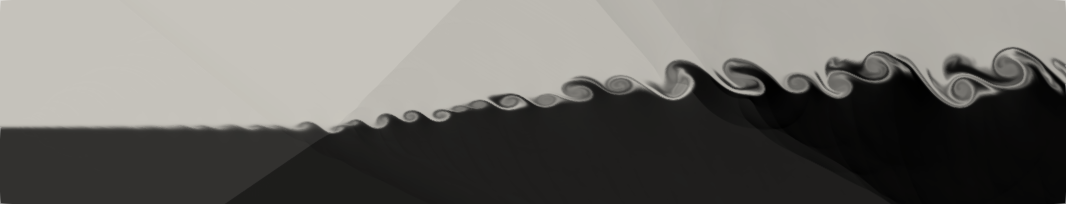
\includegraphics[width=0.99\columnwidth]{figs/mach-1-crop.png}
\caption{Case \#1}
\label{fig:mach1}
\end{subfigure}
\begin{subfigure}{.48\textwidth}
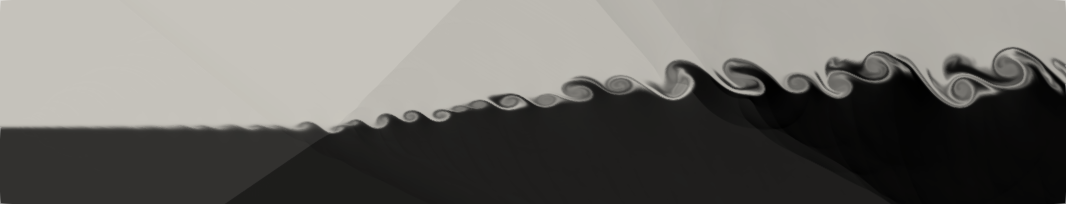
\includegraphics[width=0.99\columnwidth]{figs/mach-1-crop.png}
\caption{Case \#1}
\label{fig:mach6}
\end{subfigure}
\begin{subfigure}{.48\textwidth}
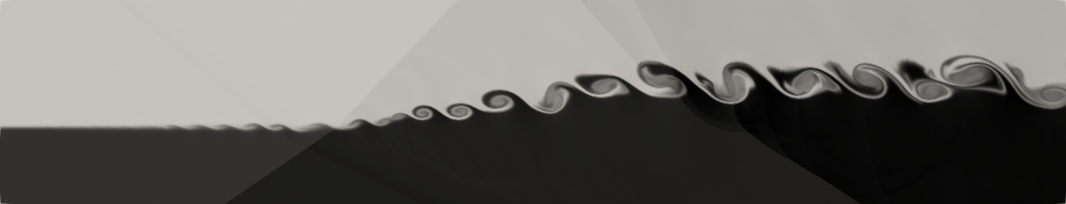
\includegraphics[width=0.99\columnwidth]{figs/mach-2-crop.png}
\caption{Case \#2}
\label{fig:mach2}
\end{subfigure}
\begin{subfigure}{.48\textwidth}
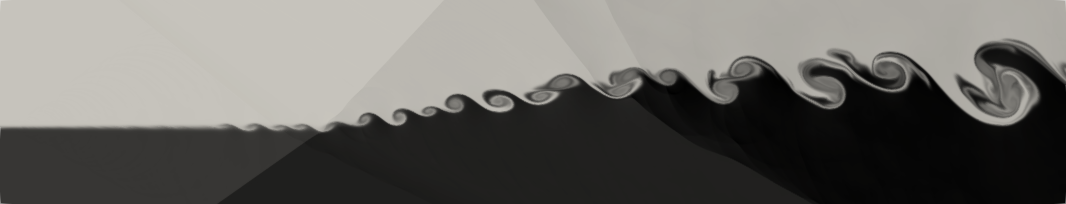
\includegraphics[width=0.99\columnwidth]{figs/mach-6-crop.png}
\caption{Case \#6}
\label{fig:mach6}
\end{subfigure}
\begin{subfigure}{.48\textwidth}
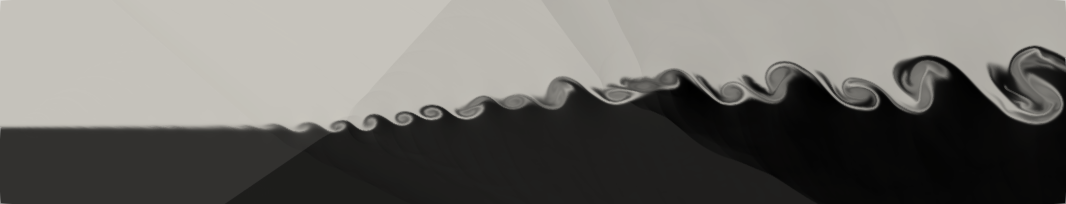
\includegraphics[width=0.99\columnwidth]{figs/mach-3-crop.png}
\caption{Case \#3}
\label{fig:mach3}
\end{subfigure}
\begin{subfigure}{.48\textwidth}
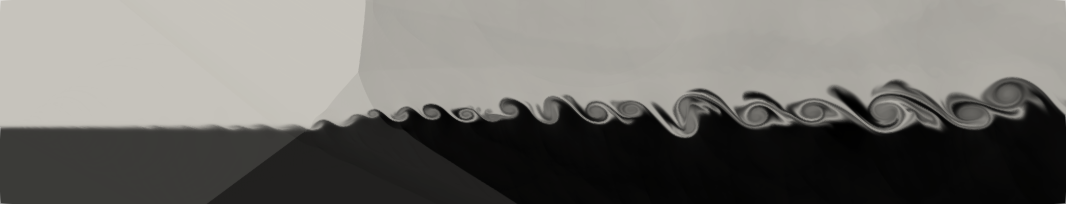
\includegraphics[width=0.99\columnwidth]{figs/mach-11-crop.png}
\caption{Case \#11}
\label{fig:mach11}
\end{subfigure}
\begin{subfigure}{.48\textwidth}
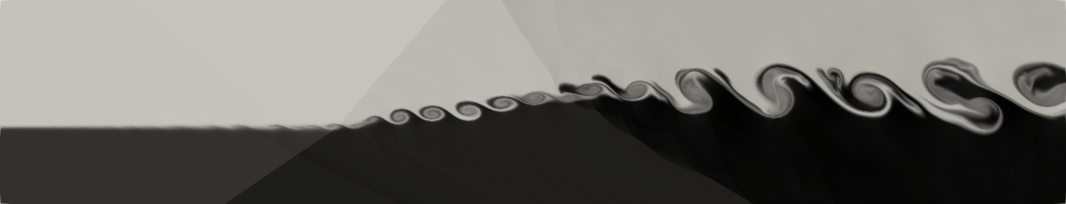
\includegraphics[width=0.99\columnwidth]{figs/mach-4-crop.png}
\caption{Case \#4}
\label{fig:mach4}
\end{subfigure}
\begin{subfigure}{.48\textwidth}
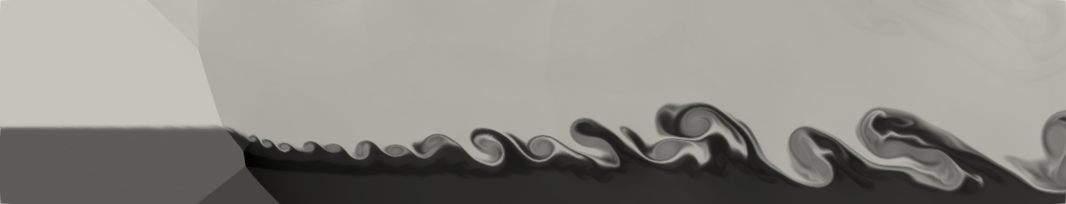
\includegraphics[width=0.99\columnwidth]{figs/mach-16-crop.png}
\caption{Case \#16}
\label{fig:mach1}
\end{subfigure}
\begin{subfigure}{.48\textwidth}
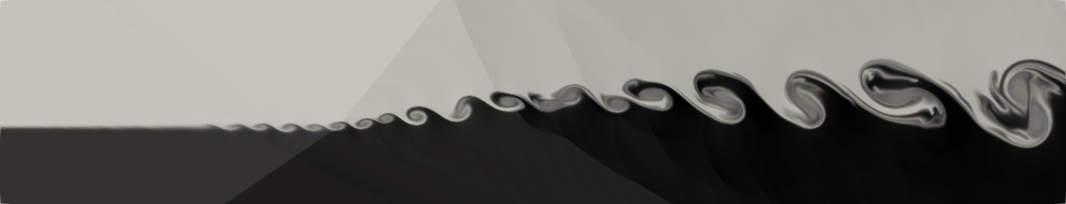
\includegraphics[width=0.99\columnwidth]{figs/mach-5-crop.png}
\caption{Case \#5}
\label{fig:mach5}
\end{subfigure}
\begin{subfigure}{.48\textwidth}
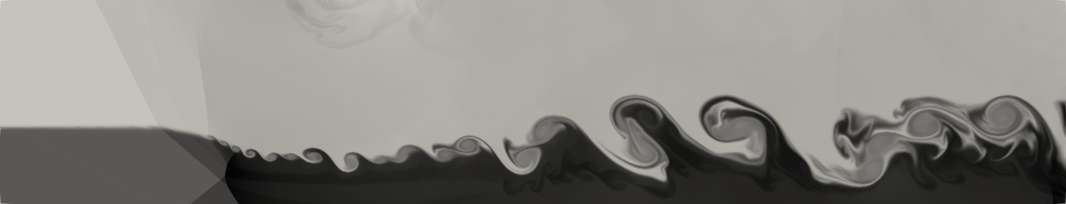
\includegraphics[width=0.99\columnwidth]{figs/mach-21-crop.png}
\caption{Case \#21}
\label{fig:mach21}
\end{subfigure}
\caption{Instantaneous field of the numerical local Mach number at $t\Delta U/\dwz= 100$ for (left panel) a fixed degree of oblique shock and for (right) fixed convective Mach number.}
\label{fig:fixedangle}
\end{figure}
%
In this left panel of this figure, it is remarkable that by increasing the convective Mach number of bulk viscosity, the normalized abscissa at which the vortex roll-up processes take place at approximately the same position.
%
The main observed difference is the position at the which the shear layer interacts with the reflected shock by the upper adiabatic wall. 
%
Moreover, the sensitivity of the growth rate with the respect to the convective Mach number does not exhibit noticeable difference.
%
However, as can be seen from the right panel of Fig.~\ref{fig:fixedangle}, the vortex structure as well the growth of the shear layer seems to be highly impacted by small perturbation of oblique shock wave. 
%
The vortex structures issued from the reflected shock interaction are indeed much more disorganized and elongated as the angle of oblique shock is intensified, and and the flow topology remains an ordered whole and the morphology of the vortices retains its coherence after the second interaction with the shock for lower values of $\beta$.

In order to quantify the growth rate of the computer shear layer, a passive scalar $\xi$ is defined on the basis of conserved elemental (\textit{i.e.}, atomic) mass fractions~\cite{pierce2001progress}.
%
The mass fraction of chemical element $\gamma$, denoted $a_\gamma$, is readily deduced from the chemical species mass fractions
%
\begin{equation}
a_{\gamma} = \sum_{\alpha=1}^{\nspc} \frac{Y_{\alpha} N_{\alpha,\gamma} A_{\gamma}}{W_{\alpha}} ,
\end{equation}
%
where $A_{\gamma}$ is the atomic weight associated to element $\gamma$ and $N_{\alpha,\gamma}$ denotes the number of $\gamma$ atoms present in each molecule of chemical species $\alpha$. For a two-feeding inlet system such as the one considered here, the mixture fraction is then obtained by summing over all elemental mass fractions and normalizing the result
%
\begin{equation}
\xi = \frac{\sum_{\gamma} |a_{\gamma} - a_{\gamma,\ce{O}}|}{\sum_{\gamma} |a_{\gamma,\ce{F}} - a_{\gamma,\ce{O}}|} ,
\label{eq:mixture-variable}
%
\end{equation}
%
where $a_{\gamma,\ce{O}}$ and $a_{\gamma,\ce{F}}$ denote the mass fractions of atom $\gamma$ in the oxidizer and fuel inlet streams, respectively.
%
The spatial evolution of the shear layer thickness $\mathbb{T}_\mathrm{sl}$ is computed as follows
%
\begin{equation}
\mathbb{T}_\mathrm{sl}=\widetilde{\xi_{0.95}}-\widetilde{\xi_{0.05}}
\end{equation}
%
\begin{figure}[!ht]
\centering
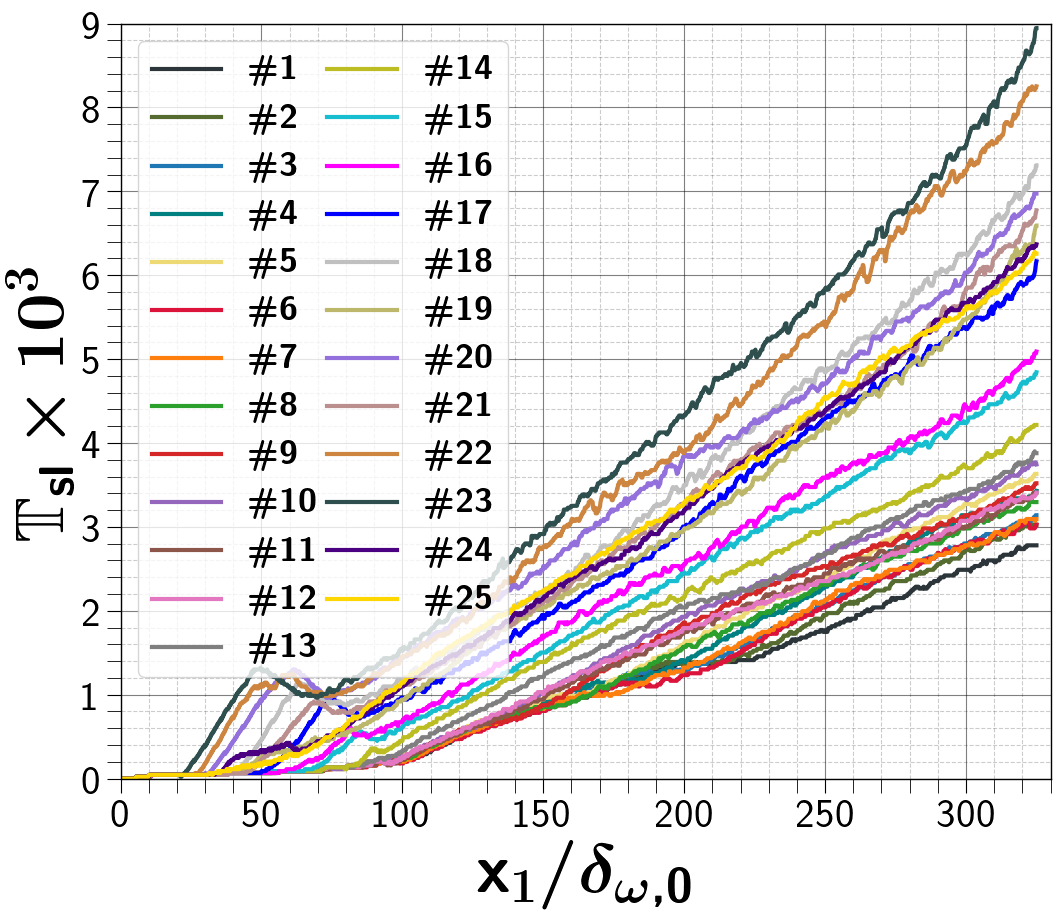
\includegraphics[width=0.50\columnwidth]{figs/xievol.png}
\caption{spatial evolution of the shear layer thickness $\mathbb{T}_\mathrm{sl}$.}
\label{fig:tslsh}
\end{figure}
%
The spatial evolution of all the cases is shown in Fig.~\ref{fig:tslsh}, which reveals that the interaction of the reflected shock wave with the mixing zone changes significantly the mixing layer growth rate with respect to the parameters $M_c$ and $\beta$.
%
For a fixed $\beta$, the thickness increases as $M_c$ goes higher. 
%
The same observation applies with a fixed $M_c$ and increasing value of $\beta$.
%

%
\begin{figure}[!ht]
\centering
\begin{subfigure}{.48\textwidth}
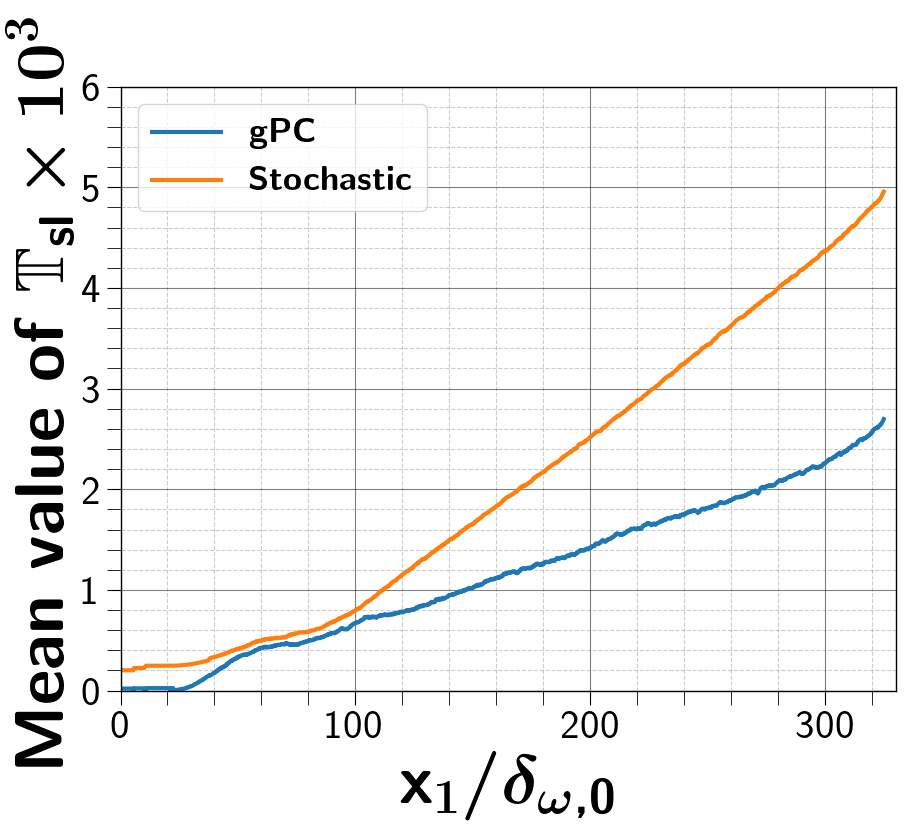
\includegraphics[width=0.99\columnwidth]{figs/meangpc.png}
\caption{}
\label{fig:mean1}
\end{subfigure}
\begin{subfigure}{.48\textwidth}
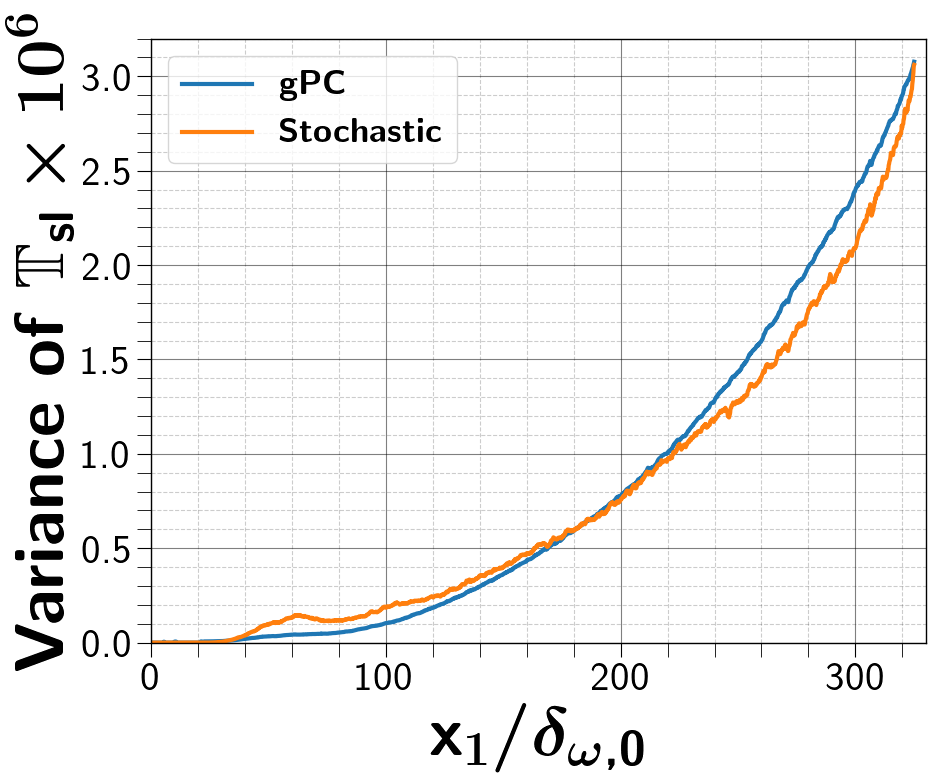
\includegraphics[width=0.99\columnwidth]{figs/vargpc.png}
\caption{}
\label{fig:mvar1}
\end{subfigure}
\caption{$\mathbb{T}_\mathrm{sl}$ mean and (b) variance solution comparison between gPC and stochastic methods.} 
\label{fig:tmeansol}
\end{figure}
%
The stochastic analysis of $\mathbb{T}_\mathrm{sl}$ is used herein to quantify the effects associated with the variability of $M_c$ and $\beta$.
%
The analysis here is performed relying on the use of the gPC to reconstruct multiple response surfaces, considering a uniform $\texttt{PDF}$ for the input parameters $M_c$ and $\beta$.
%
The comparison obtained from the gPC and the stochastic methods is highlighted in Fig.~\ref{fig:mean1}.
%
The stochastic method over-estimates the mean value of the gPC method in the fully turbulent region, which indicates that the gPC was not able to capture the mean field.
%
This means that, under the current operational point, the gPC method requires more polynomial degree, and therefore more computational efforts should be deployed to obtain its convergence.
%
The uncertainty depicted by the parameters is more likely to explain the non-convergence of the gPC.
The variance of $\mathbb{T}_\mathrm{sl}$ with respect to its mean value in the parameter space is provided in Fig.~\ref{fig:mvar1}.
%
As expected, the variance increases as the fully developed turbulent region is reached.
%
Unlike the mean value, the values of variance computed by means of the gPC is well compared to the stochastic method, even though the convergence of gPC is not obtained.
%
It is noteworthy that an estimation of the sensitivity will allow to rank the parameters depending on their sensitivity. 
%

%
\begin{figure}[!ht]
\centering
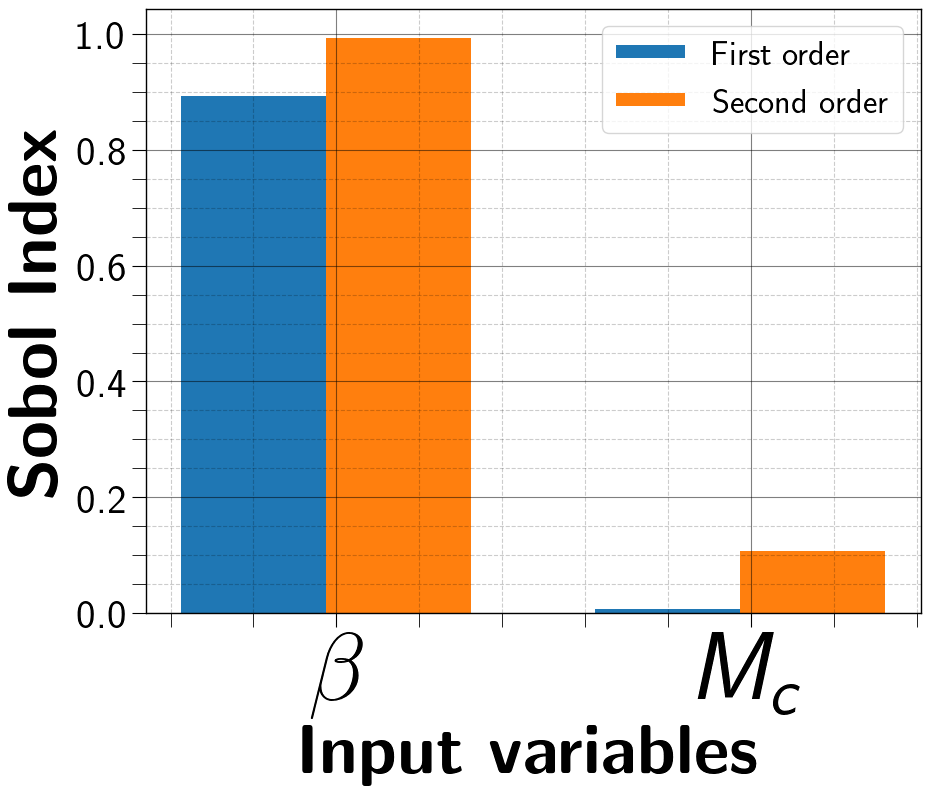
\includegraphics[width=0.49\columnwidth]{figs/sobol.png}
\caption{The Sobol indices for $\mathbb{T}_\mathrm{sl}$} 
\label{fig:tmeansobol}
\end{figure}
%
The analysis of the Sobol indices for  $\mathbb{T}_\mathrm{sl}$ is depicted in Fig.~\ref{fig:tmeansobol}.
%
One can note that the uncertainty is totally controlled by angle of the oblique shock wave, which 
indicates that that there is no coupling between the effects of $\beta$ and $M_c$, resulting in a  response dictated mainly by the quantity $\beta$ in the parameter space.
%
The Total Sobol’ Indices show the existence of an uncertainty resulting from the interaction of $\beta$ and $M_c$, but the interaction does not impact the overall sensitivity analysis.
%
As a conclusion, one can limit uncertainty quantification on the uncertainty of $\beta$. 
%=============================================================
\section{Conclusion}
%=============================================================
In this study, a sensitivity analysis of DNS of the shocked turbulent spatially evolving mixing layer has been performed. The effects of the convective Mach number $M_c$ and the angle of oblique shock wave have been investigated.
%
The choice of the parameters is performed with the aim to improve the physical understanding of the considered flow configuration.
%
This naturally opens up interesting prospects for flow control, and reliable comparison between experiments, simulations and turbulence modelling.
%
A database of 25 two-dimensional DNS has been used to perform the analysis, which encompassed observation of structural features as well as stochastic characterization of time-averaged quantities.
%
The latter has been developed via response surface reconstruction using gPC.
%
The response surface reconstruction allows for an accurate quantification of the effects of each parameter, as well as of the total variation rate in the parametric range investigated.
%
The main finding of this work is that for uncertainty quantification could be limited to the study of the uncertainty of $\beta$.
%
Future work envisions the investigation of the effects of $\beta$-angle in combination with different inlet perturbations, in particular for the initial development of the mixing layer. The impact of variations of the Reynolds number could also be addressed. 
%=========================================================
\paragraph{Acknowledgements}
%=========================================================
The authors gratefully acknowledge support and computing resources from the African Supercomputing Center (ASCC) at UM6P (Morocco).
%=============================================================
\bibliography{main}
%=============================================================
\end{document}